\documentclass{article}
\usepackage[utf8]{inputenc}
\usepackage{amsmath}
\usepackage{enumitem}
\usepackage{graphicx}
\usepackage{framed}
\usepackage{listings}
\usepackage{pdfpages}
\usepackage{caption}
\usepackage{subcaption}
\usepackage[utf8]{inputenc}
\usepackage{minted}
\usepackage{placeins}
\usepackage[utf8]{inputenc}
%\usepackage[english]{babel}
 
% \usepackage[
% backend=biber,
% style=alphabetic,
% sorting=ynt
% ]{biblatex}

\usepackage{natbib}
%\setcitestyle{authoryear,open={((},close={))}}
 
% \addbibresource{main.bib}


\title{Ch 10 Group}
\author{Tate Meehan, Arash Modaresi Rad, William Rudisill}
\date{March 2019}

\begin{document}

\maketitle

\section*{Equation}
The Van Genuchten equation is used to model volumetric soil water content as a function of pressure head \citep{dingman} : 
\begin{align}
\theta = \theta_r + \frac{\theta_s - \theta_r}{\big(1 + \alpha h^n\big)^m}
\end{align}

\section*{Part 1 -- Apply the GN with explicit second-order regularization using the L-curve.}
The GN method is given by:
\begin{equation}
\mathbf{K}\left(\mathbf{m}^{(k)}\right)^{T} \mathbf{K}\left(\mathbf{m}^{(k)}\right) \Delta \mathbf{m}=-\mathbf{K}\left(\mathbf{m}^{(k)}\right)^{T} \left[ \begin{array}{c}{\mathbf{G}\left(\mathbf{m}^{(k)}\right)-\mathbf{d}} \\ {\alpha \mathbf{L} \mathbf{m}^{(k)}}\end{array}\right]
\end{equation}
Where $\alpha$ is a regularization parameter that we choose. Selecting the $\alpha$ entails weighting the desired parameter smoothness constraint to find a solution that minimizes the residual of the fit between the model and the data. The code takes different number of iterations to converge depending on the alpha value chosen. Figure \ref{fig:iterations} shows the number of iterations versus the alpha value. The "optimal" $\alpha$ value is approximately .24. Figure \ref{fig:solutions} shows various solutions for different $\alpha$ values.   


\begin{figure}[ht!]
    \centering
    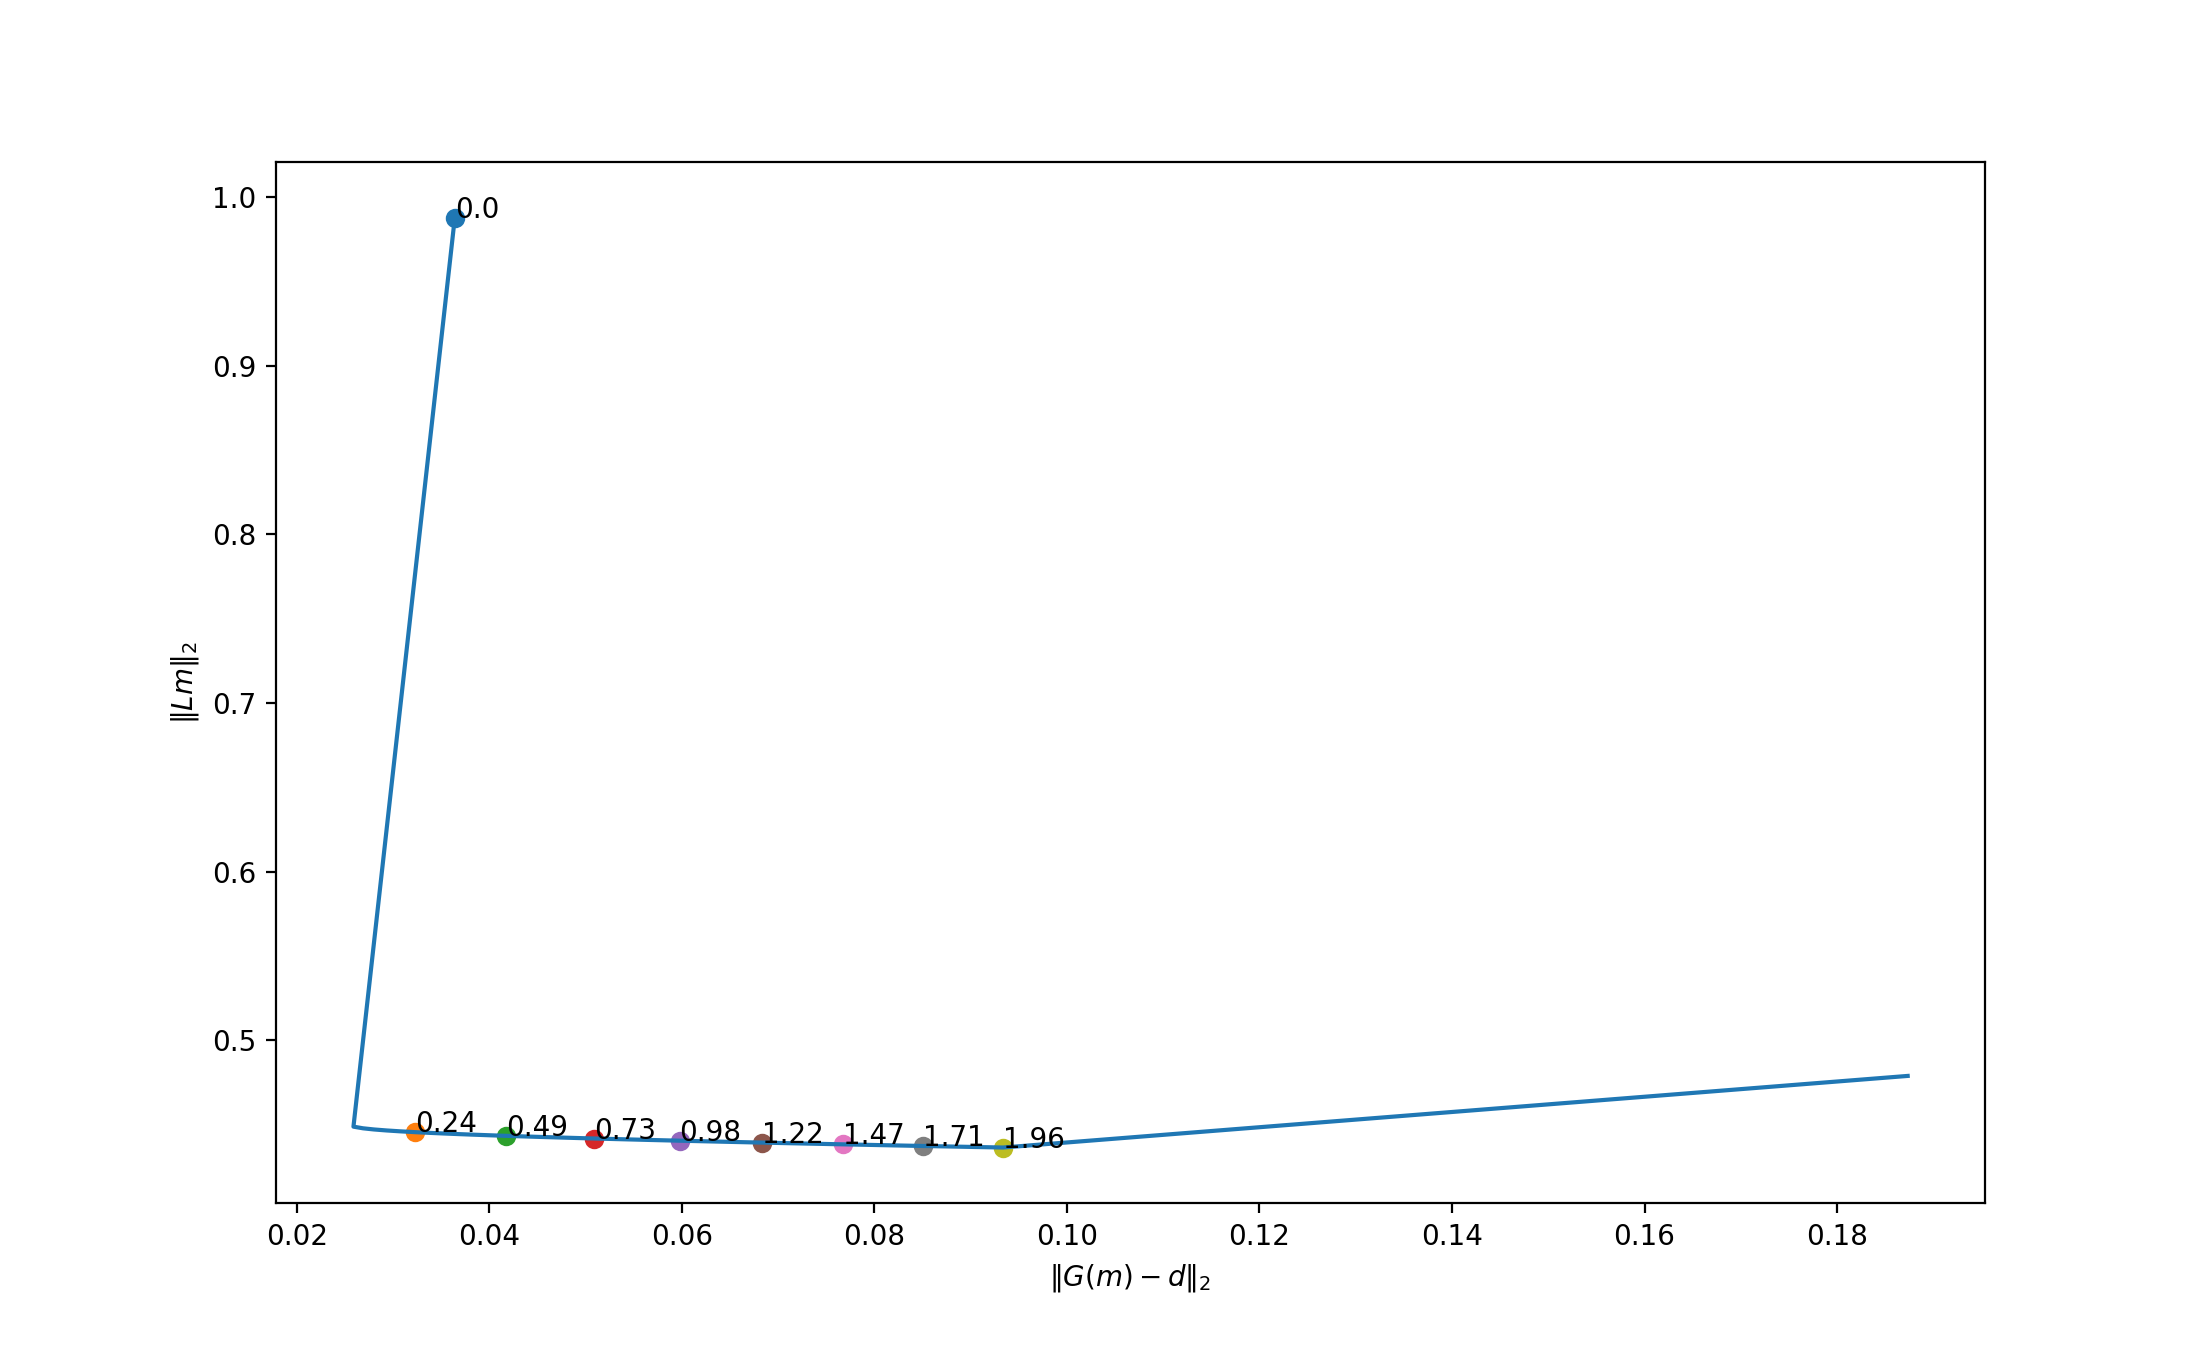
\includegraphics[width=4.5in]{LCurve_GNmethod.png}
    \caption{The L-Curve for the GN Method. Alpha values range between 0 and 2.0. Selected alpha values are labelled on the L-curve. The "optimal" $\alpha$ is approximately .24}
    \label{fig:lcurve}
\end{figure}


\begin{figure}[ht!]
    \centering
    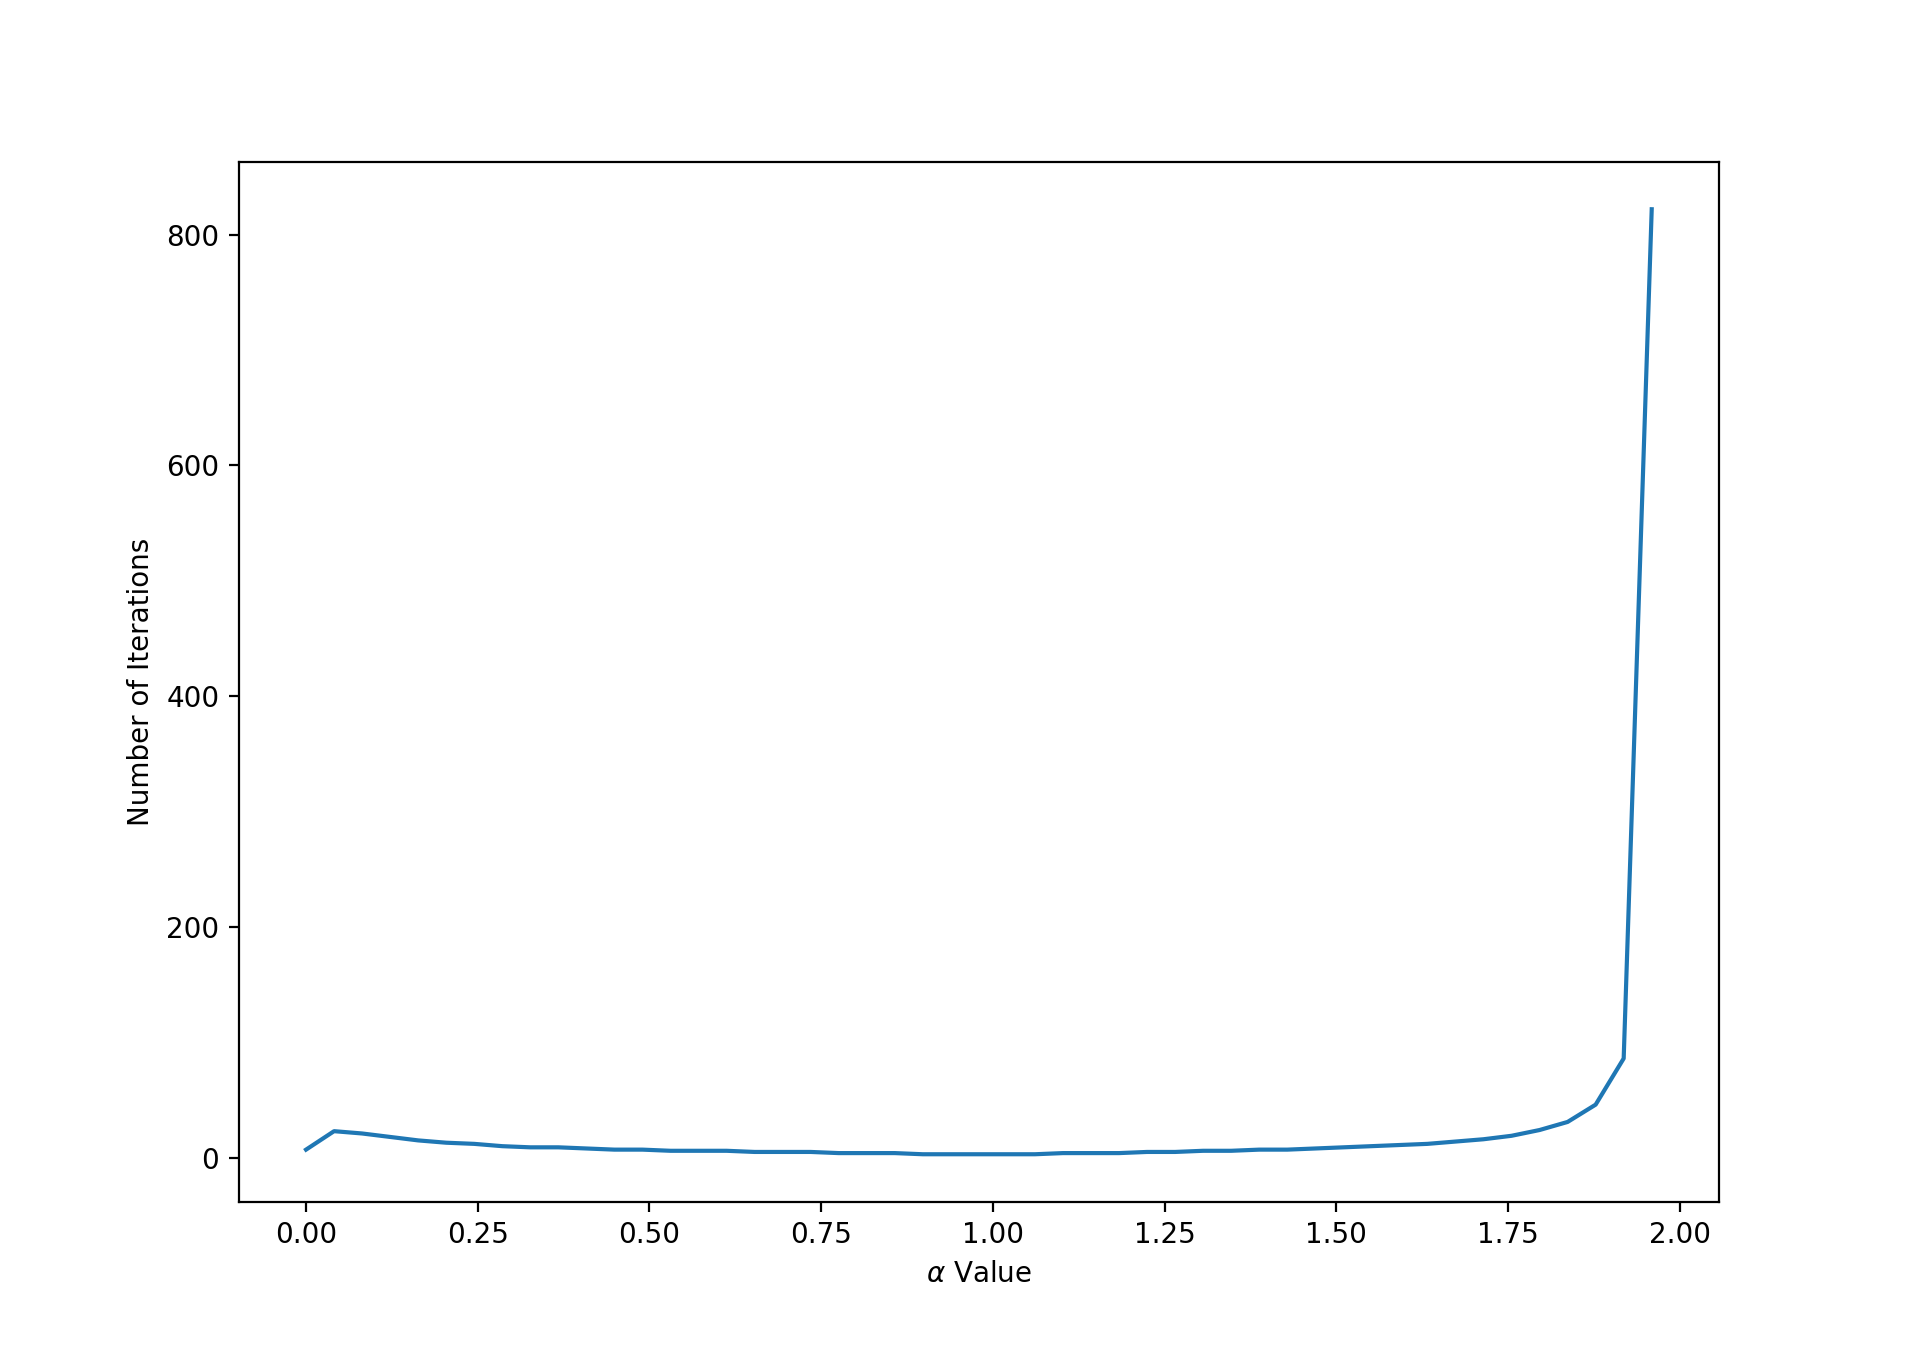
\includegraphics[width=4.5in]{Iterations_Alphas.png}
    \caption{The number of iterations to convergence (defined in text) versus the alpha parameter}
    \label{fig:iterations}
\end{figure}


\begin{figure}[ht!]
    \centering
    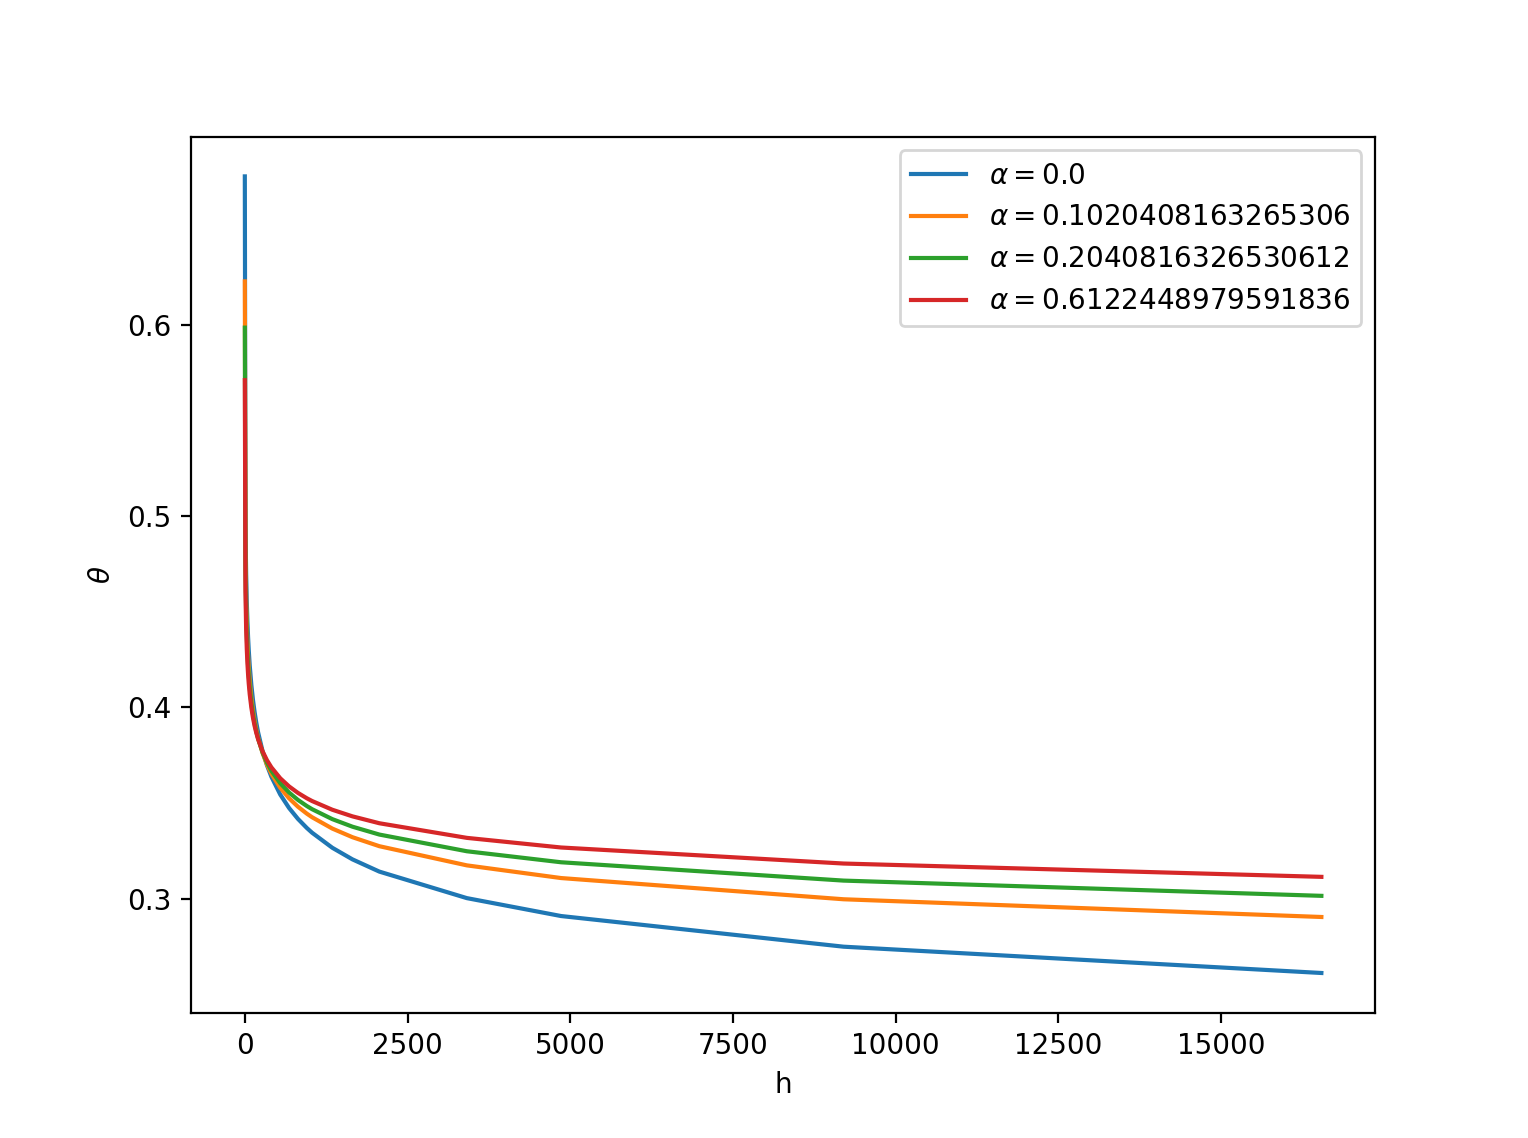
\includegraphics[width=4.5in]{alphas_range_plot.png}
    \caption{Various solutions with different values of $\alpha$}
    \label{fig:solutions}
\end{figure}
\FloatBarrier
\section*{Part 2 -- Apply Occam's method with explicit second-order regularization using the discrepancy principle.}
\subsection*{a. Identify a value of delta, and justify your choice.}

The value for delta was chosen following the discrepancy principle where $\Delta^2$ is the $95^{th}$ percentile of the $\chi^2$ distribution with $\nu = m - n = 23$ degrees of freedom.

\subsection*{b. Graph the value of chi-squared with your chosen value of alpha as a function of the iteration k.}
\begin{figure}
    \centering
    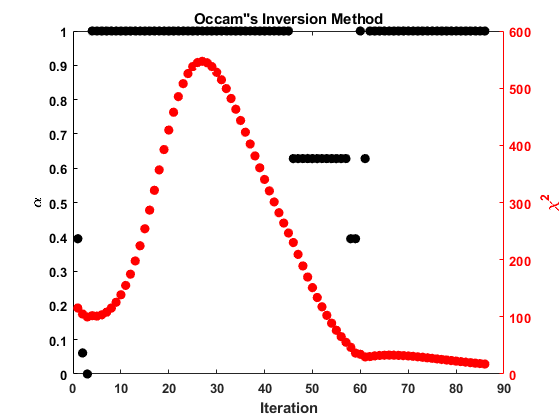
\includegraphics[width = \textwidth]{2bb.png}
    \caption{Wthin Occam's inversion method, the alpha value is adjusted per iteration (shown in black). The $\chi^2$ value of the solution is plotted in red. Our chosen convergence criteria was set by two conditions: $\frac{\|m^{k-1}-m^{k}\|}{\|m^{k}\|} > 1e-3$ and $\chi^2 > \frac{1}{2}\Delta^2$.}
    \label{fig:2b}
\end{figure}

\subsection*{c. Report the parameters at the final iteration, and the number of iterations it took to converge.}
The solution recovered in Figure \ref{fig:2c} required 86 iteration to converge as shown in Figure \ref{fig:2b}. The parameters recovered at the $86^{th}$ iterate are presented in Table \ref{tab:2}.
\begin{table}[!h]
\begin{center}
\begin{tabular}{|c|c|c|c|c|}
\hline
$\alpha = \mathbf{m_1}$ & $n = \mathbf{m_2}$ & $m = \mathbf{m_3}$ & $\theta_S = \mathbf{m_4}$ & $\theta_R = \mathbf{m_5}$ \\ \hline
$0.0122$                & $0.6348$           & $0.8237$           & $0.5508$                  & $0.456$                   \\ \hline
\end{tabular}
\caption{The solution to the van Genuchten equation for a random starting guess.}
\label{tab:2}
\end{center}
\end{table}


\begin{figure}
    \centering
    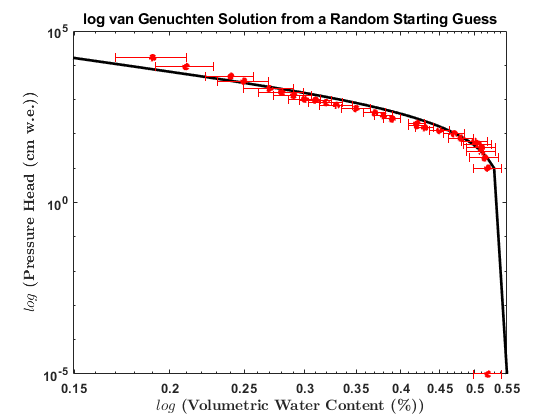
\includegraphics[width = 0.85\textwidth]{2logvanG.png}
    \caption{The estimated van Genuchten solution from the data points shown in log space. The accepted parameters bare little physical accuracy, although the solution satisfies the convergence criteria.}
    \label{fig:2c}
\end{figure}
\FloatBarrier

\section*{Part 3 -- Apply regularization with prior estimates of the parameters and their standard deviations.}
\subsection*{a. Justify your choice of initial parameter values and their corresponding standard deviations}
We chose parameters for $m_prior$ from the literature that matched our informed estimate of the soil type. We then chose standard deviation values that are proportional to the magnitude of the parameter value. We modified the GN method to incorporate the initial parameter estimates and standard deviations as follows:


\begin{equation}
\mathbf{K}\left(\mathbf{m}^{(k)}\right)^{T} \mathbf{K}\left(\mathbf{m}^{(k)}\right) \Delta \mathbf{m}=-\mathbf{K}\left(\mathbf{m}^{(k)}\right)^{T} \left[ \begin{array}{c}{\mathbf{G}\left(\mathbf{m}^{(k)}\right)-\mathbf{d}} \\ {\alpha \mathbf{L} ( \frac{\mathbf{m}^{(k)} - \mathbf{m_0}}{m_{\sigma}})}\end{array}\right]
\end{equation}


We found reasonable behaviour using the GN method with the prior parameter estimate and standard deviations. Figure \ref{fig:alpha_m_prior} shows the two norm residual between the inverse parameter solution, m, and the prior parameter estimate $m_0$. Unsurprisingly, as the alpha value increases, the difference between the solution and the prior parameter estimate decreases.


\begin{figure}
    \centering
    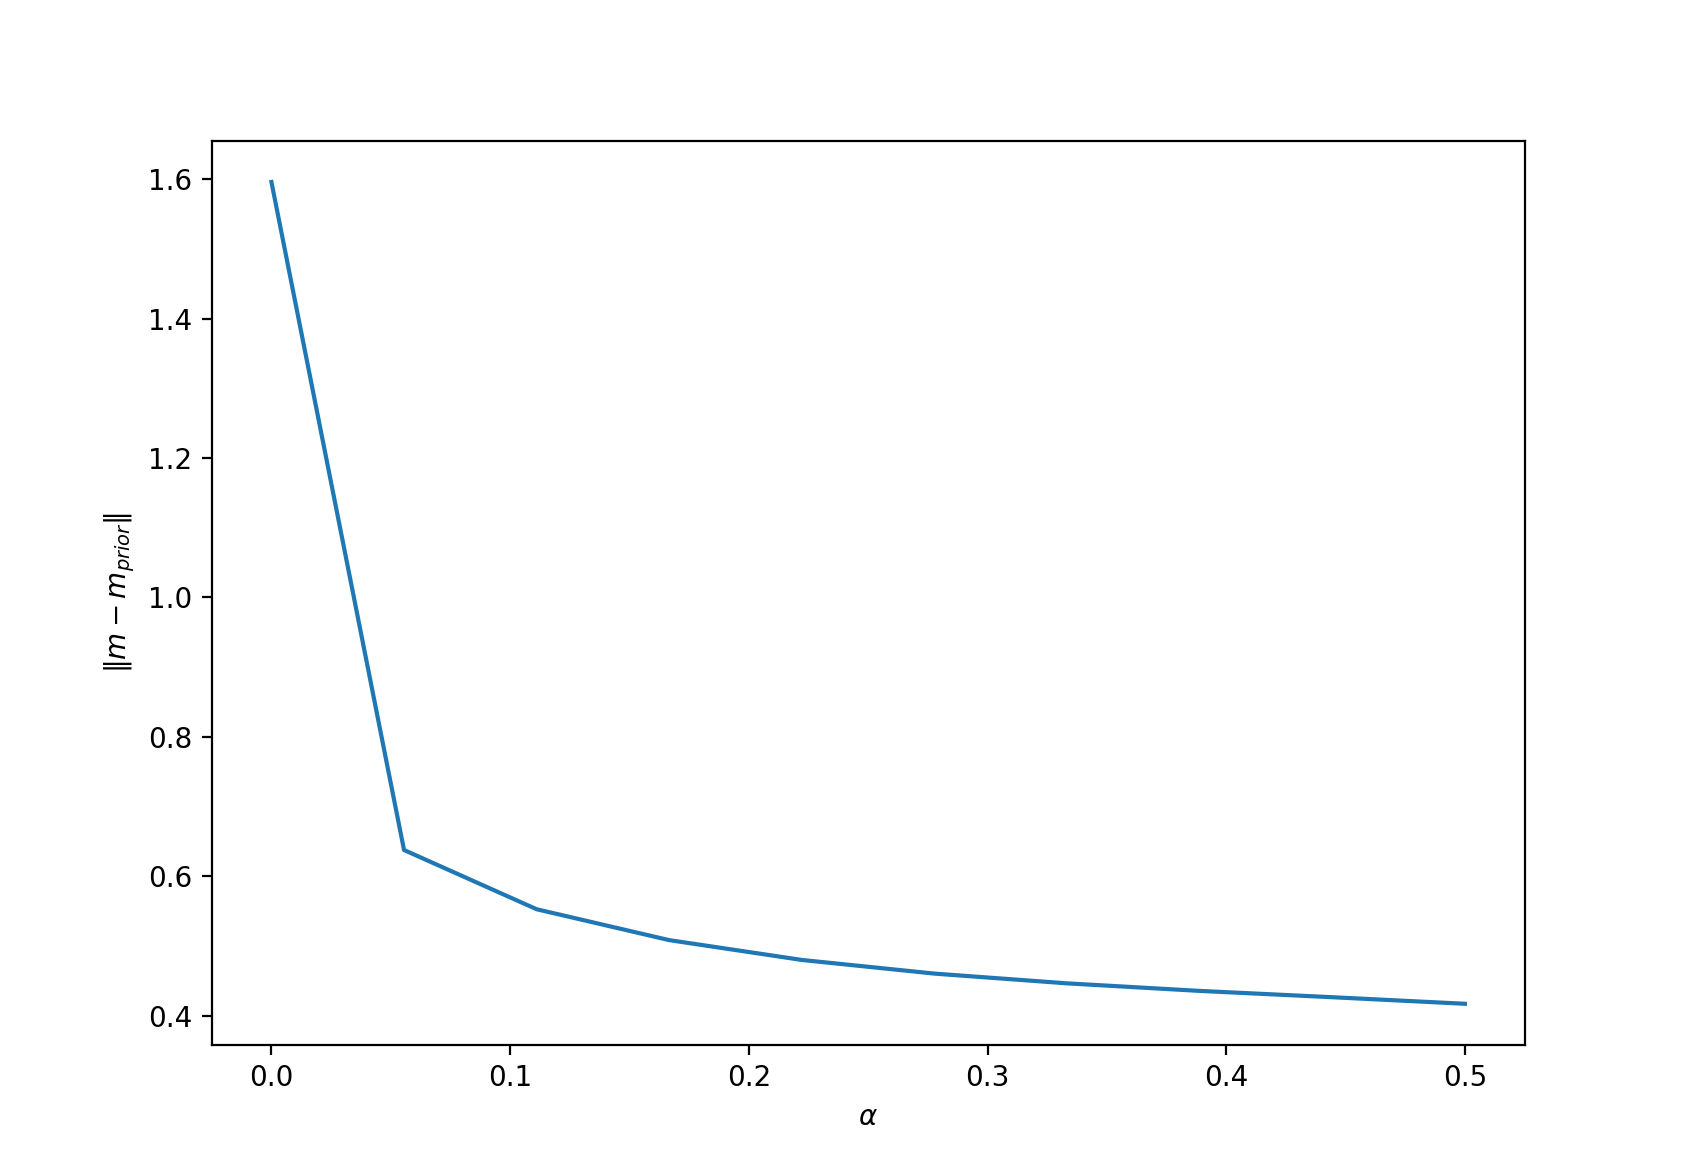
\includegraphics[width=4in]{m_prior_alpha.png}
    \caption{$\alpha$ versus the 2-norm difference between the inverse solution and the 'prior' parameter estimate.}
    \label{fig:alpha_m_prior}
\end{figure}

\subsection*{b. \textbf{Report the parameters at the final iteration, and the number of iterations it took to converge}}
\begin{table}[!h]
\centering
\begin{tabular}{|c|c|c|c|c|c|}
\hline
& $\theta_R\mathbf{m_5}$ & $\theta_S \mathbf{m_4}$ & $\alpha = \mathbf{m_1}$ & $n = \mathbf{m_2}$ & $m = \mathbf{m_3}$ \\
\hline
Prior & .86 & .04 & .033 & 1.49 & .33 \\
Recovered & .452 & .057 & .063 & 1.55 & .381 \\
\hline
\end{tabular}
\end{table}


The solution took 425 iterations to converge to a solution using and alpha value of .5. The iterations decreased as the alpha value was increased. Prior parameter values were takin from \citet{hillel2005}.


\section*{Part 4 -- Compare the accuracy of your results from 1-3 and their computational effort}

We found that in the GN method there exists a single loop that calls to the partial derivatives and model functions, whereas the Occam's method calculates the forward model and the Jacobian in the outer loop and then within the inner loop it calculates the $\chi^2$ every time. Therefore, the GN method is computationally more efficient than the Occam's.
The accuracy can be described as the trade off between regularization term added to the objective function and the residuals. However, since we do not know the true parameters of the model and utilizing goodness of fit criteria such as root mean square error would only indicate the misfit based on residuals, the accuracy of the results is unknown.


\section*{Part 5 -- Choose the best parameter estimates from 1-3}
We have chosen the results from part 3 as the best parameter estimates, because the solution parameters are most close to their physical representation by soil classification. Although an acceptable fit is achieved by any of the methods, the solution parameters do not necessarily agree with the published values for the particular soil type.
\subsection*{\textbf{What is the resolution of your estimates?}}
If we interpret 'resolution' as the ability to recover model parameters with a particular physical meaning, then our model in fact has quite poor resolution. In a 'perfect world', where the Van Genuchten model exactly describes reality, then the data (pressure and volumetric water content) would uniquely describe a set of parameters, and these parameters would correspond with physical soil properties that quantifiable. However, through the inversion, we find many suitable parameter sets that correspond with a wide range of different soil characteristics (not shown, but as found in the literature). So, in this way, the inversion has a poor resolution. 
\subsection*{\textbf{Are there any problems with local minima?}}
Yes. We did not rigorously test it, but we found that the starting parameter set could have an impact on the final parameter estimate for the Occam's and GN methods. Considering that there were many suitable parameter sets for this particular soil data, we can argue that our least square problem is not well-conditioned and the Van Genuchten model may be a physically unreasonable model in this case.

\bibliographystyle{abbrvnat}
\bibliography{main.bib}

\section*{Appendix}

\begin{minted}{matlab}
%% Group Assignment Chapter 10
% Tate Meehan, Arash Modaresi, Will Rudisill
clear; close all; clc;
%% 
addpath('C:\Users\snowfield\Desktop\Backup\Math\Inverse Theory\PEIP-code\Lib');
global theta;
global h;
global sigma;
[h] = xlsread('soil.xlsx','sheet1','B2:B29');
m = length(h);
theta = xlsread('soil.xlsx','sheet1','C2:C29');
dev = xlsread('soilstd.xlsx','sheet2','F2:F29');
dev = [NaN;dev];
sigma = inpaint_nans(dev,1);
% sigma = std(theta);
% sigma = 1;
h(1) = 0.00001;
% p0 = ([1,1,1,.6,.1]');
% Parameters from table
% m = 1/(exp(.182)-1)
% p0 = [exp(-2.076),exp(.182),1,.482,.090]';
% Guess with Weighting
% p0 = ([.01,1,1,1,1]')./2;
% Randon Starting Guess
p0 = [2.*rand, 5.*rand, rand, rand, rand]';
% p0 = [0.033 1.49 0.33 0.48 0.123]';
% load('goodGuess.mat')
n = length(p0);
tol = eps.^(.125);
maxiter = 1000;

% Discrepancy Principle
% sigma = .035; % Estimate of Data Standard Deviation
% delta = sigma.*sqrt(m);
delta = sqrt(chi2inv(0.95,m-n));

L2 = full(gallery('tridiag',n,-1,2,-1));
% L2 = eye(n);

[pstar, alphachi, iter] = occam('vanGenuchten', 'jac', L2, theta, p0, delta);
% [pstar, iter] = lm('fun', 'jac', p0, 0.0001, maxiter);

goodWill =  vanGenuchten(pstar);

% % Posterior Standard Deviation Estimate
dof = length(h) - 5;
% s = norm(goodWill - theta)./sqrt(dof);

figure();plot((goodWill),(h),'k','linewidth',2);
hold on; errorbar((theta),(h),(ones(length(theta),1).*sigma./2),'horizontal','or','markerfacecolor','r','markersize',5);
xlabel('Volumetric Water Content (%)')
ylabel('Pressure Head (cm w.e.)')
set(gca,'fontweight','bold')
% figure();plot(log(goodWill),log(h),'k','linewidth',2);
% hold on; errorbar(log(theta),log(h),(ones(length(theta),1).*s./2),'horizontal','or','markerfacecolor','r');

figure();plot((goodWill),(h),'k','linewidth',2);
hold on; errorbar((theta),(h),(ones(length(theta),1).*sigma./2),'horizontal','or','markerfacecolor','r','markersize',5);
set(gca, 'XScale','log', 'YScale','log')
xlabel('\textbf{$log$ (Volumetric Water Content (\%))}','interpreter','latex')
ylabel('\textbf{$log$ (Pressure Head (cm w.e.))}','interpreter','latex')
set(gca,'fontweight','bold')

figure(); yyaxis left ;plot(1:length(alphachi),alphachi(:,1),'ok','markerfacecolor','k','linewidth',1); ylabel('\alpha')
yyaxis right; plot(1:length(alphachi),alphachi(:,2),'or','markerfacecolor','r','linewidth',1); ylabel('\chi^2'); xlabel('Iteration')
title('Occam"s Inversion Method')
set(gca,'fontweight','bold')
ax = gca;
ax.YAxis(1).Color = 'k';
ax.YAxis(2).Color = 'r';
% % Report the chi2 Value
% chi2 = sum(((goodWill - theta)./s).^2);
% % Report the p value
% p = chi2cdf(chi2,dof);
% 
% % Compute the Covariance and Correlation Matrecies
% J=jac(pstar);
% covm = s.^2.*inv(J'*J);
% sig = sqrt(diag(covm));
% corrm = covm./(sig*sig');
% confinterval = tinv(0.975,dof).*diag(covm).^.5;

% Parameter Estimation and Inverse Problems, 3rd edition, 2018
% by R. Aster, B. Borchers, C. Thurber
% m=occam(fun,jac,L,d,m0,delta)
%
% INPUT
%   fun   - a function handle that computes the forward problem
%   jac   - a function handle that computes the Jacobian of the forward problem
%   L     - a regularization matrix
%   d     - the data that should be fit
%   m0    - a guess at the model
%   delta - the cutoff to use for the discrepancy principle portion
%
% OUTPUT
%   m - the model found
%
function [m, out, iter] = occam(fun, jac, L, d, m0, delta)
m = m0;
oldm = zeros(size(m));
iter = 0;
mchi2 = 2.*delta^2;
global sigma


% while we have not converged sufficiently or the data misfit is higher than
% allowed keep iterating
while (norm(oldm-m) / norm(m) > 1e-3) || (mchi2 > delta^2.*.5)
    % only allow 1000 iterations
    iter = iter + 1;
    if (iter > 1000)
        return;
    end
    
    % store the old mode to test for convergance
    oldm = m;
    
    % get the current data that would be generated and the jacobian
    G = feval(fun, m);
%     if norm(d - G)^2 > 5.*sigma.*sqrt(length(G))
%         m = [2.*rand, 5.*rand, rand, rand, rand]';
%         G = feval(fun, m);
%     end
    J = feval(jac, m);
    
    % get the dhat that is in equation 10.14
        dhat = d - G + J * m;

%     if iter == 1
%     dhat = d - G + J * m;
%     else
%     dhat = d - G + J * (m-m0);
%     end

    
    % This is a simple brute force way to do the line search.  Much more
    % sophisticated methods are available.  Note: we've restricted the line
    % search to the range from 1.0e-20 to 1.  This seems to work well in
    % practice, but might need to be adjusted for a particular problem.
    
    alphas = logspace(-20, 0, 100);
    for ii = 1:100
        M = J' * J + alphas(ii)^2 * (L' * L);
        
        % if M is not terribly conditioned
        try
        if (cond(M) < 1.0e15)
            m = M \ (J' * dhat);
            
            % store the associated data misfit
%             chis(i) = norm(feval(fun, m)-d, 2)^2;
            chis(ii) = norm((feval(fun, m)-d)./sigma, 2)^2;

        else
            % M behaves poorly enough it should not be used
            chis(ii) = + Inf;
        end
        catch
            chis(ii) = + Inf;
        end
    end
    
    [Y, I] = min(chis);
    
    if (Y > delta^2)
        %disp('Improving Chi^2');
        alpha = alphas(I(1));
    else
        %disp('Smoothing m');
        I = find(chis <= delta^2);
        alpha = alphas(max(I));
    end
    
    % store the new model and misfit
    m = (J' * J + alpha^2 * L' * L) \ J' * dhat;
%     m = abs(real(m));
%     mchi2 = norm(feval(fun, m)-d, 2)^2;
    mchi2 = norm((feval(fun, m)-d)./sigma, 2)^2;
    
    out(iter,:) = [alpha, mchi2]; 
    

end

% Computes the Jacobian of fun for the slug test Example 9.1
% from Parameter Estimation and Inverse Problems, 3rd edition, 2018
% by R. Aster, B. Borch(ii)ers, C. Th(ii)urber
% 
% p is expected to be a five element vector
%   [a, n, m, thetaS, thetaR]
%
function J=jac(p)
% global variables, these are 
% theta, h
global theta;
global h;
global sigma;

% use known formula for the derivatives in the Jacobian
nn=length(theta);
J=zeros(nn,2);
for ii=1:nn
    % Recalculated with Weights
    J(ii,1) = -(p(2).*p(3).*abs(h(ii)).*(p(4)-p(5)).*(p(1).*abs(h(ii))).^(p(2)-1).*((p(1).*abs(h(ii))).^(p(2)) + 1).^(-p(3)-1))./sigma(ii);
    J(ii,2) = -(p(3).*log(p(1).*abs(h(ii))).*(p(4)-p(5)).*(p(1).*abs(h(ii))).^(p(2)).*((p(1).*abs(h(ii))).^(p(2)) + 1).^(-p(3)-1))./sigma(ii);
    J(ii,3) = -(log((p(1).*abs(h(ii))).^(p(2))+1).*(p(4)-p(5)).*((p(1).*abs(h(ii))).^(p(2))+1).^(-p(3)))./sigma(ii);
    J(ii,4) = 1./(sigma(ii).*((p(1).*abs(h(ii))).^(p(2))+1).^(p(3)));
    J(ii,5) = (1./sigma(ii)) - 1./(sigma(ii).*((p(1).*abs(h(ii))).^(p(2))+1).^(p(3)));

% Unweighted
%     J(ii,1) = -(p(2).*p(3).*abs(h(ii)).*(p(4)-p(5)).*(p(1).*abs(h(ii))).^(p(2)-1).*((p(1).*abs(h(ii))).^(p(2)) + 1).^(-p(3)-1));
%     J(ii,2) = -(p(3).*log(p(1).*abs(h(ii))).*(p(4)-p(5)).*(p(1).*abs(h(ii))).^(p(2)).*((p(1).*abs(h(ii))).^(p(2)) + 1).^(-p(3)-1));
%     J(ii,3) = -(log((p(1).*abs(h(ii))).^(p(2))+1).*(p(4)-p(5)).*((p(1).*abs(h(ii))).^(p(2))+1).^(-p(3)));
%     J(ii,4) = 1./(1.*((p(1).*abs(h(ii))).^(p(2))+1).^(p(3)));
%     J(ii,5) = (1./1) - 1./(1.*((p(1).*abs(h(ii))).^(p(2))+1).^(p(3)));

% Orignal Form
%   J(ii,1)= (p(4)-p(5)).*(-p(1).*h(ii).^2.*p(3).*(p(2)).*abs(p(1).*h(ii)).^(p(2)-2)...
%       .*(abs(p(1).*h(ii)).^(p(2))+1).^(-p(3)-1));
%   J(ii,2)= (p(4)-p(5)).*(-p(3).*abs(p(1).*h(ii)).^(p(2)).*log(abs(p(1).*h(ii)))...
%   .*(abs(p(1).*h(ii)).^(p(2))+1).^(-p(3)-1));
%   J(ii,3)= (p(4)-p(5)).*(-(abs(p(1).*h(ii)).^(p(2))+1).^(-p(3)).*log(p(1).*h(ii)).^(p(2))+1);
%   J(ii,4) = 1./((1+abs(p(1).*h(ii)).^p(2)).^p(3));
%   J(ii,5) = 1 - 1./((1+abs(p(1).*h(ii)).^p(2)).^p(3));
end

% Computes the differences between forward model prediction and data,
% normalized by the standard deviation for the slug test Example 9.1.
% from Parameter Estimation and Inverse Problems, 3rd edition, 2018
% by R. Aster, B. Borchers, C. Thurber
%
% fvec=fun(p)
%
%
% p is expected to be a five element vector
%   [a, n, m, thetaS, thetaR]
function fvec = vanGenuchten(p)
% global variables, these are 
global theta
global h
% Compute the function values.
fvec=zeros(length(theta),1);
for i=1:length(theta)
%   fvec(i)= (p(5) + (p(4) - p(5))./((1+(abs(p(1).*h(i)).^p(2))).^p(3)));
  fvec(i)= (p(5) + (p(4) - p(5))./((1+(p(1).*abs(h(i)).^p(2))).^p(3)));

end  

\end{minted}





\end{document}



